\begin{figure}[H]
\centering
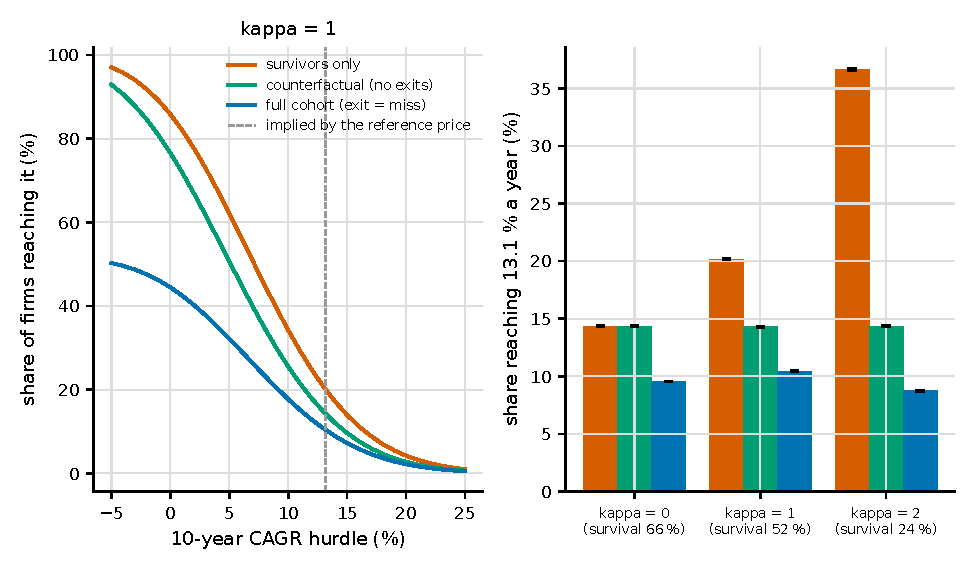
\includegraphics[width=0.74\linewidth]{figures/fig27_base_rates.pdf}
\caption{How often is the growth implied by the reference price achieved? Synthetic universe of the v0.4 survivorship study (2000 cohorts of 2000 firms, 10 years; FCF growth compared with revenue growth, i.e. a constant FCF margin assumed). Left: the three base rates against the CAGR hurdle (exit hazard strength kappa = 1). Right: at the implied growth, for exits unrelated to growth (kappa = 0) and increasingly growth-driven exits; error bars $\pm 1.96$ se. A database of today's survivors overstates the chance of a firm picked today.}
\label{fig:fig27_base_rates}
\end{figure}
